\begin{figure}[h]
	\centering
	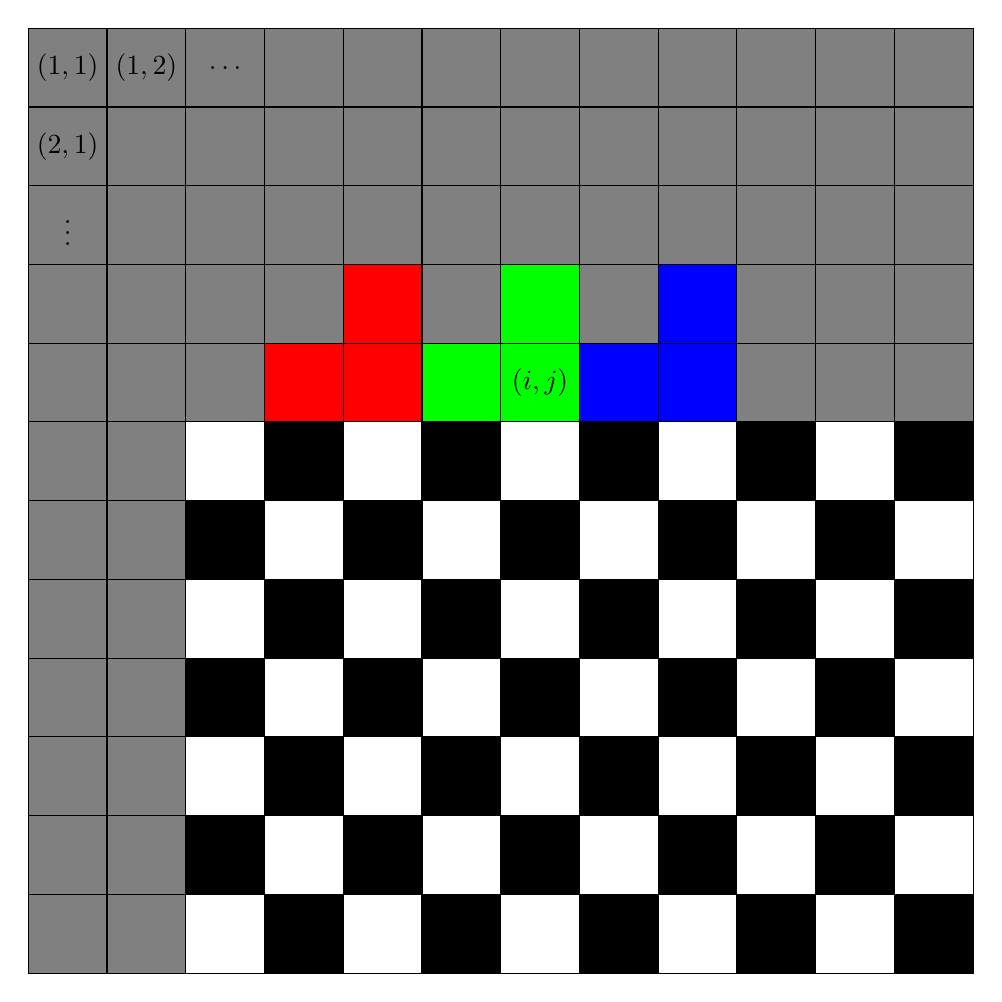
\begin{tikzpicture}
		\foreach \i in {-6, ..., 5}
			\foreach \j in {-6, ..., 5}
				\filldraw[gray] (\i, \j) rectangle + (1, 1);
		\foreach \i in {-4, ..., 5}
			\foreach \j in {-6, ..., 0}
				{
					\pgfmathparse{mod(\i+\j, 2) ? "black" : "white"}
					\edef\colour{\pgfmathresult}
					\filldraw[fill=\colour] (\i, \j) rectangle + (1, 1);
				}
		\foreach \x in {(-2, 1), (-3, 1), (-2, 2)}
			\filldraw[red] \x rectangle + (1, 1);
		\foreach \x in {(0, 1), (-1, 1), (0, 2)}
			\filldraw[green] \x rectangle + (1, 1);
		\foreach \x in {(2, 1), (1, 1), (2, 2)}
			\filldraw[blue] \x rectangle + (1, 1);
		\draw[step=1] (-6, -6) grid (6, 6);
		\node at (0.5, 1.5) {$(i, j)$};
		\node at (-5.5, 5.5) {$(1, 1)$};
		\node at (-4.5, 5.5) {$(1, 2)$};
		\node at (-3.5, 5.5) {$\dots$};
		\node at (-5.5, 4.5) {$(2, 1)$};
		\node at (-5.5, 3.5) {$\vdots$};
	\end{tikzpicture}
	\caption{The random variable $\norm{\Delta^- F(i, j)}$ only depends on the green pixels, $\norm{\Delta^- F(i, j - 2)}$ depends on the red pixels and $\norm{\Delta^- F(i, j + 2)}$ on the blue pixels. Since these are all distinct from another, the random variables are independent.}
	\label{fig: independentpoints}
\end{figure}